% The Planner Is the Adversary — draft v0.2 (retargeted framing, 2026-07-06).
% Idea-of-record: diagnosis/docs/PAPER_IDEA.md (update pending); every claim maps
% to a row in diagnosis/docs/CLAIMS_EVIDENCE.md (C1–C7) — do not add claims
% without a row there. E0 overoptimization numbers (C5.3) are RUNNING (SLURM
% 24740/24741); their table/figure slots are marked \todo and must not ship
% until n=8 lands. Previous Boundary-Blindness-led draft: git history (v0.1).
%
% Build: pdflatex main && bibtex main && pdflatex main && pdflatex main
\documentclass[10pt]{article}
\usepackage[margin=1in]{geometry}
\usepackage{amsmath,amssymb,amsfonts}
\usepackage{booktabs}
\usepackage{graphicx}
\usepackage{multirow}
\usepackage{xcolor}
\usepackage[colorlinks=true,linkcolor=blue,citecolor=blue,urlcolor=blue]{hyperref}
\usepackage[round]{natbib}

\newcommand{\todo}[1]{\textcolor{red}{[TODO: #1]}}
\newcommand{\bb}{\mathrm{BB}}

\title{The Planner Is the Adversary: Test-Time Search Exploits Learned Costs in
Latent World-Model Planning}

\author{%
  Anonymous\thanks{Draft v0.2, 2026-07-06 (retargeted). Sections 3--5 and 7
  carry final numbers (see \texttt{diagnosis/results/} and
  \texttt{diagnosis/docs/CLAIMS\_EVIDENCE.md}); Section 6.2 (overoptimization
  curves) is running and marked TODO.}}
\date{}

\begin{document}
\maketitle

% ======================================================================
\begin{abstract}
Action-conditioned JEPA world models plan by test-time search: at every control
step, a sampling optimizer (CEM) scores hundreds of imagined futures with a
learned cost and executes the best candidate. We show that on contact-rich
manipulation this coupling --- an optimizer pitted against a learned proxy ---
is where planning fails, and that the dominant and previously unmeasured failure
mode is \emph{cost overoptimization} (Goodhart's law) rather than merely missing
information. All experiments use frozen pretrained checkpoints. Two kinds of numbers recur: \emph{planning success}, counted as
successful episodes out of 16 (written $k/16$), and \emph{readout accuracy}, the
percentage of frames whose decoded object position falls within the 5\,cm
task-success radius.
\textbf{(1)~Diagnosis.} We measure action grounding with counterfactual ranking
accuracy (CRA): given a real transition, does the predictor place the executed
action's imagined future closer to the observed next state than the futures it
imagines for 16 distractor actions? Chance is $1/17\approx 6\%$. Against
distractors drawn from similar states, every model sits at the chance floor in
contact regimes --- and the result is flat across a $45\times$ encoder scale-up
(DINOv2 22M $\to$ V-JEPA-2-AC 1B).
\textbf{(2)~Localization.} An \emph{oracle ladder} fixes the planner and its
budget, gives it \emph{perfect dynamics} (every candidate action sequence is
rolled in the simulator and encoded by the real frozen encoder), and varies only
the cost. With the true simulator-state cost, the same planner solves push
$16/16$; with every cost computed from the frozen representation it solves at
most $2/16$. Even repairing the object readout on exactly the frames the planner
scores (readout accuracy $78\%\to91.5\%$) adds \emph{zero} successful episodes.
\textbf{(3)~Mechanism.} The planner is the adversary: on the elite candidates
CEM converges to, the same readout that is $91.5\%$ accurate on random frames
drops to $24\%$ --- the search seeks out precisely the frames the cost
mis-scores, and executed plans read ``at goal'' while the true object sits
$13$--$30$\,cm away. Sweeping the search budget makes this monotone in
optimization pressure: proxy improving, true outcome flat, readout error on the
elites growing --- a Goodhart curve with an honest-cost control that, in
contrast, converts search into success. Mitigations from the
reward-hacking playbook --- readout hardening, encoder-LoRA fine-tuning (5
seeds), ensemble disagreement penalties --- all stay at $\leq 2/16$, even while
readout accuracy reaches $94$--$100\%$: \emph{grounding does not buy planning}.
Overoptimization curves confirm the mechanism is monotone in search budget, and
a search-free amortized controller --- removing the optimizer entirely --- also
fails ($0/8$), exposing a second, independent wall: the frozen representation.
Grounding is necessary, not sufficient.
\textbf{(4)~The predictor-side lever.} An action-counterfactual InfoNCE
objective (a $0.5$M-parameter predictor-LoRA, no object labels) lifts CRA on
real-robot DROID data from the $6\%$ chance floor to $61\%$ and cuts a
planning-probe action error by $26\%$, while \emph{improving} reconstruction.
The implication for evaluation: prediction accuracy and grounding metrics do not
predict plannability; world models intended for planning should report the
cost's \emph{exploitability under the planner's own optimization pressure}.
\end{abstract}

% ======================================================================
\section{Introduction}

Action-conditioned world models that predict in a learned latent space --- the
JEPA family (DINO-WM~\citep{zhou2024dinowm}, V-JEPA-2-AC~\citep{assran2025vjepa2},
and the design study of~\citet{jepawms2025}) --- plan by coupling two learned
components with a test-time optimizer: a predictor imagines futures, a cost
scores them against a goal, and a sampling planner (CEM) searches for the action
sequence that minimizes the cost. On free-space tasks this works well. But a
consistent pattern runs through the field's own evaluations: the \emph{positive}
closed-loop numbers are for reaching and pose control, while contact-rich tasks
--- pushing, grasping, pick-and-place --- are omitted, demoted to qualitative
figures, or propped up with hand-crafted sub-goals. \citet{jepawms2025} stop
their closed-loop Metaworld tables at Reach and note the model ``hallucinates
grasping the object''; \citet{assran2025vjepa2} report pick-and-place only after
supplying three manual sub-goal images.

The field's implicit diagnosis is a \emph{model-capacity} story: the encoder is
too small, the representation too coarse, the predictor too weak --- scale will
fix it. This paper argues, and then shows with a chain of controlled
experiments, that the binding failure is somewhere else entirely: \textbf{in the
optimizer--cost interface}. A CEM planner at test time is an optimizer pitted
against a learned proxy objective. The reinforcement-learning-from-human-feedback
literature has a name for what happens to optimizers pitted against learned
proxies: \emph{overoptimization}, or Goodhart's law --- push on a proxy hard
enough and the true objective decouples from it~\citep{gao2023overopt,
skalse2022defining, karwowski2024goodhart, amodei2016concrete}. We show the same
phenomenon governs latent world-model planning, with one aggravating difference:
in RLHF the optimizer is a training loop one can regularize; here the optimizer
runs \emph{at every control step}, on frames the cost was never fit on, selected
adversarially \emph{because} the cost mis-scores them.

Three features distinguish our account from the classic ``model exploitation''
concern in model-based RL~\citep{janner2019trust, lambert2020objective}, where a
policy exploits errors in learned \emph{dynamics}. (i)~We give the planner
\emph{perfect dynamics} --- every candidate action sequence is rolled in the
simulator and re-encoded by the real frozen encoder --- and the failure persists
unchanged; the exploited component is the \emph{cost}, cleanly isolated.
(ii)~We show the exploitation is \emph{irreducible} for the frozen-encoder
regime: a ladder of increasingly strong cost repairs (better formula, better
readout, off-policy hardening, encoder fine-tuning, ensembling) all fail the
same way. (iii)~We show the standard diagnostic quantities the field might use
to catch this --- prediction error, action-grounding scores, readout precision
--- are all satisfied while planning fails, i.e.\ the failure is invisible to
current evaluation practice.

Concretely, our experimental chain (Metaworld with simulator ground truth for
supervision and verification; DROID for real-robot transfer) is:

\begin{itemize}
  \item \textbf{C1 (diagnosis at scale, Sec.~\ref{sec:diagnostic}).} On frozen
  checkpoints, action grounding against \emph{nearest-neighbour} action
  distractors sits at the chance floor ($\approx 0.059$) in every
  contact-relevant regime,
  and our Boundary-Blindness instrument shows the models smear exactly the
  contact bifurcations that decide a grasp. Crucially this is
  \emph{scale-invariant}: flat across a $45\times$ encoder scale-up and two
  self-supervised families, up to and including V-JEPA-2-AC at 1B parameters.
  \item \textbf{C2 (the wall, at upstream parity, Sec.~\ref{sec:planning}).} Our
  closed-loop harness reproduces the published Metaworld Reach baseline
  ($6/16 = 37.5\%$, CI $[18.5, 61.4]\%$, vs.\ the reported $44.8\pm8.9\%$), and
  both the $L_2$ and grounded planners score $0/16$ on push and pick-and-place
  with a diagnostic signature: the arm arrives ($2$--$4$\,cm from its goal
  pose), the object never moves.
  \item \textbf{C3 (localization: the oracle ladder, Sec.~\ref{sec:ladder}).}
  Swapping one component per rung under perfect dynamics: the true-state cost
  solves push $16/16$; latent-$L_2$, object-readout, learned-metric, and
  probe-based state costs collapse to $0$--$2/16$. A measured repair of the
  off-policy readout ($78\!\to\!91.5\%$ within $5$\,cm on the exact frame
  distribution CEM scores) transfers \emph{zero} planning success --- readout
  precision was never the binding constraint.
  \item \textbf{C4 (mechanism: the planner is the adversary,
  Sec.~\ref{sec:adversary}).} CEM's converged elite population decodes at
  $24\%$ within $5$\,cm versus $91.5\%$ on random off-policy frames --- the
  search specifically finds and converges onto the cost's error pockets, driving
  the object to where the cost reads ``at goal'' while it is $13$--$30$\,cm
  away. Sweeping the search budget makes this a Goodhart curve monotone in
  optimization pressure --- proxy improving, true outcome flat, elite readout
  error growing --- with an honest-cost control (reach) that instead turns search
  into success ($2/8\to8/8$). Mitigations from the reward-hacking playbook ---
  hardened readouts, encoder-LoRA (5 seeds), ensemble disagreement penalties,
  relearned representation adapters --- all stay within the frozen baseline's
  $0$--$2/16$, even at $94$--$100\%$ grounding: \emph{grounding does not buy
  planning}.
  \item \textbf{C5 (removing the adversary is not sufficient,
  Sec.~\ref{sec:e1}).} A search-free amortized controller (goal-conditioned
  inverse dynamics on the same frozen representation) also solves push $0/8$, and
  re-adding search in doses corrupts its plans at a rate rising with dose
  ($0\to7\%$) but never crosses the wall --- the object never moves. Contact
  planning faces \emph{two} walls: the exploitable cost/optimizer interface and
  an insufficient frozen representation. Grounding is necessary, not sufficient.
  \item \textbf{C6 (the axis that moves, Sec.~\ref{sec:cf}).} An
  action-counterfactual InfoNCE objective on the predictor (LoRA, $0.5$M
  parameters, no object labels) improves DROID Action-Error in all six
  regime$\times$horizon cells (pooled $1.468\!\to\!1.086$, $-26\%$) and lifts
  effect-conditioned action grounding from chance ($0.061$) to $0.605$, while
  improving reconstruction --- the training-side counterpart of the analysis,
  and the correct level at which to intervene on the \emph{predictor} axis.
\end{itemize}

\paragraph{Conventions (how to read our numbers).}
Four kinds of quantities appear throughout, and we keep their formats distinct.
\emph{Planning success} is always episodes solved out of 16 paired evaluation
episodes, written $k/16$ (with the percentage in parentheses when comparing to
published baselines). \emph{Readout accuracy} is always the percentage of
frames whose decoded object position falls within the $5$\,cm task-success
radius (``$\%$ within $5$\,cm''), with the median error in cm where informative.
\emph{CRA} is a ranking accuracy over transitions, reported as a fraction in
tables; with $16$ distractors, chance is $1/17 \approx 0.059$. \emph{AUG/ECS}
are raw latent-space gaps (Sec.~\ref{sec:metrics}), meaningful only within a
model. Distances in the workspace are in cm or in Metaworld state units where
noted.

The through-line is a reframing of what world-model evaluation must report.
Prediction error is satisfied while planning fails (Sec.~\ref{sec:diagnostic});
grounding is satisfied while planning fails (Sec.~\ref{sec:adversary});
readout precision is satisfied while planning fails (Sec.~\ref{sec:ladder}).
The quantity that tracks the failure is the gap between what the cost claims
and what the world delivers \emph{on the states the optimizer converges to} ---
the cost's exploitability under optimization pressure. We propose it as a
first-class evaluation axis for world models intended for planning.

% ======================================================================
\section{Related work}\label{sec:related}

\paragraph{JEPA world models for planning.}
DINO-WM~\citep{zhou2024dinowm} predicts forward in the frozen feature space of a
self-supervised image encoder and plans with sampling-based MPC from a goal
image; V-JEPA-2-AC~\citep{assran2025vjepa2} learns an action-conditioned world
model on a video encoder and demonstrates zero-shot manipulation;
\citet{jepawms2025} systematically study the design choices that make such
models plan. We take these as frozen baselines and treat their own evaluations
as evidence: across all three, strong closed-loop results are pose/free-space
tasks, and contact is where the story thins (hand-crafted sub-goals, qualitative
figures, ``hallucinated grasping''). Our work explains why the wall sits
precisely at contact and why it does not yield to scale.

\paragraph{Overoptimization and reward hacking.}
Optimizing against a learned proxy eventually decouples proxy from truth:
formalized for RLHF reward models by~\citet{gao2023overopt}, characterized
in general by~\citet{skalse2022defining} and~\citet{karwowski2024goodhart},
and anticipated as ``reward hacking''~\citep{amodei2016concrete}. We port this
lens to latent-space planning, where it has not been quantitatively
established: the CEM inner loop is the optimizer, the latent cost is the proxy,
and the elite population is the analogue of the over-optimized policy. Our
oracle ladder gives this port an isolation the RLHF setting lacks --- we can
hold dynamics \emph{perfect} and vary only the cost.

\paragraph{Model exploitation in model-based RL.}
That policy optimization exploits errors in learned \emph{dynamics} is a classic
MBRL concern~\citep{janner2019trust}, related to the objective mismatch between
likelihood training and control performance~\citep{lambert2020objective}.
Our finding is materially different: with dynamics oracle-controlled, the
\emph{cost} is exploited at test time --- a failure that persists when the
dynamics-error channel is closed entirely, and that standard dynamics-side
remedies (ensembles, pessimism) do not touch (Sec.~\ref{sec:adversary}).

\paragraph{Concurrent diagnostics and objectives.}
Concurrently, ATM~\citep{atm2026} proposes a post-hoc action-identifiability
diagnostic for frozen latent world models with a training-time supervision fix,
and UWM-JEPA~\citep{uwmjepa2026} shows in a physics toy setting that
teacher-forced JEPA objectives admit action-invariant solutions which
counterfactual targets repair --- independently confirming the mechanism behind
our Sec.~\ref{sec:cf} objective. Neither work addresses planning: our
contributions beyond both are the planner-level exploitation analysis
(Secs.~\ref{sec:ladder}--\ref{sec:adversary}), the scaling study, and the
demonstration on pretrained robot world models at up to 1B parameters.
IMWM~\citep{imwm2026} observes that finite-budget sampling planners can be the
bottleneck even under an idealized world model and responds with demonstration
priors; \citet{latentgeom2026} amortize planning into an inverse-dynamics
controller, removing test-time search --- a direction our analysis independently
motivates as \emph{removing the adversary} (Sec.~\ref{sec:discussion}).
Vision-tactile world models~\citep{contactworld2026} address what information
contact planning needs; our results say that adding information without
addressing exploitability is not sufficient (Sec.~\ref{sec:ladder}).

\paragraph{Benchmarks.}
We evaluate on Metaworld~\citep{yu2020metaworld}, whose simulator state lets us
supervise and \emph{verify} costs against ground truth, and
DROID~\citep{khazatsky2024droid} as the real-robot transfer check. Planning
follows the upstream CEM configuration~\citep{rubinstein1997cem}.

% ======================================================================
\section{Diagnosis: action grounding is at chance and does not scale}
\label{sec:diagnostic}

We first establish, on frozen checkpoints (nothing trained), that the
contact-regime action grounding the planner would need is absent --- and that
this is not a capacity artifact. This section compresses the diagnostic
instrument; full definitions and the AUG/ECS corroboration are in
App.~\ref{app:bb} and App.~\ref{app:augecs}.

\subsection{Metrics}\label{sec:metrics}
Let $F(z,a)$ be the frozen one-step latent predictor (driven through the
model's own \texttt{unroll} primitive, with the model's own action
normalisation) and $d$ the upstream planning distance ($L_2$ for every
baseline, matching the shipped \texttt{L2\_cem} configuration). We measure
three complementary quantities on held-out factual transitions
$(z_t, a_t, z_{t+1})$; each answers a different question.

\textbf{CRA --- does the model rank the executed action best?} Given the
transition, we sample $K{=}16$ distractor actions $\{a^-_k\}$ and ask whether
the factual action's prediction lands closer to the realised next latent than
every distractor's prediction:
\begin{equation}
  \mathrm{CRA} = \Pr\!\Big[\, d\big(F(z_t,a_t),z_{t+1}\big) <
       \min_{k=1\ldots K} d\big(F(z_t,a^-_k),z_{t+1}\big) \Big],
\end{equation}
so chance is $1/(K{+}1) = 1/17 \approx 0.059$. The distractor family controls
what the metric tests: \emph{opposite} distractors ($a^- = -a_t$) test coarse
directional grounding --- the quantitative version of the ``open vs.\ close the
gripper'' visualisations in prior work --- while \emph{nearest-neighbour}
distractors are actions \emph{actually executed} from the $K$ most similar
latent states in the dataset: plausible alternatives a competent policy might
take from this state, so ranking the factual action above them requires
resolving exactly the fine action differences planning depends on. Being a
ranking, CRA is comparable across models with different latent scales; it is
our primary cross-model metric.

\textbf{AUG --- does the action help at all?} The Action Usage Gap is the
prediction-error increase when the action is replaced by another action from
the batch (a permutation $\pi$):
\begin{equation}
  \mathrm{AUG} = \mathbb{E}\big[\, d\big(F(z_t,\pi(a_t)),z_{t+1}\big)
                          - d\big(F(z_t,a_t),z_{t+1}\big)\,\big],
\end{equation}
which is $\approx 0$ if and only if the predictor ignores its action input.
AUG is a raw latent-space gap: informative \emph{within} a model, not
comparable \emph{across} models (latent scales differ), which is why it
corroborates CRA rather than replacing it (App.~\ref{app:augecs}).

\textbf{ECS --- the same question, asked where it matters.} Averaged over all
transitions, AUG can be diluted by near-static steps (the arm hovering; the
scene unchanged) where different actions genuinely lead to similar futures.
Effect-Conditional Sensitivity restricts AUG --- and, in the
\emph{effect-conditioned CRA} we report as the primary signal, the ranking ---
to transitions that actually move the latent, $\|z_{t+1}-z_t\| > \tau$ with
$\tau$ the per-model median displacement. A low effect-conditioned score
therefore reflects genuine action-ignoring, not quiet data.

\textbf{Boundary Blindness} ($\bb$; definition in App.~\ref{app:bb}) is our
fourth instrument, answering a question none of the above can: is the model's
action-sensitivity \emph{calibrated to the world's}? On a neighbourhood of
similar states, it compares how much the \emph{world's} true outcomes fan out
under nearby actions against how much the \emph{model's} predictions fan out
under the same actions, both z-scored over the population; $\bb > 0$ means the
world bifurcates (e.g.\ grasp vs.\ miss) while the model predicts nearly the
same future for every nearby action. Because $\bb$ references ground-truth
outcomes, a high value cannot be explained away by small one-step latent
deltas.

\textbf{Protocol.} Transitions are stratified into four regimes --- free
space, pre-grasp, gripper actuation, contact manipulation --- via a proxy from
the Metaworld simulator state (object displacement as the contact signal;
DROID uses proprioception and latent-change heuristics). All confidence
intervals are trajectory-clustered bootstrap. Every frame is encoded once and
cached; nothing is trained for the diagnostic.

\subsection{Frozen baselines fail on nearby actions, at the boundary}
\begin{table}[h]
\centering\small
\caption{Effect-conditioned CRA (top-1, $n_{\mathrm{eff}}$-weighted pool,
Metaworld). Against \emph{opposite} distractors the models are near-perfect ---
they use actions. Against \emph{nearest-neighbour} distractors they collapse,
worst at pre-grasp: they cannot resolve the \emph{small} action differences
that decide a grasp.}
\label{tab:cra}
\begin{tabular}{llccc}
\toprule
model & distractor & free space & \textbf{pre-grasp} & contact \\
\midrule
\multirow{2}{*}{DINO-WM} & opposite          & 0.990 & 0.961 & 0.975 \\
                         & nearest-neighbour & 0.566 & \textbf{0.467} & 0.481 \\
\midrule
\multirow{2}{*}{JEPA-WM} & opposite          & 0.993 & 0.972 & 0.984 \\
                         & nearest-neighbour & 0.635 & \textbf{0.541} & 0.571 \\
\bottomrule
\end{tabular}
\end{table}

Boundary Blindness explains and localizes the collapse: pooled
$\bb_{\mathrm{boundary}}$ concentrates at the pre-grasp boundary on both model
families (DINO-WM $1.323$, JEPA-WM $1.280$, vs.\ free-space $0.28$--$0.30$;
per-task CI-aware pairing elevated in 4/6 and 5/6 tasks with zero confident
reversals) and transfers to real-robot DROID data ($1.975$ $[1.601, 2.350]$
under the $\|\Delta z\|$ proxy). The predictor is a conditional-mean estimator
under full-latent $L_2$; where contact bifurcates the outcome fan, it predicts
the fan's mean.

\subsection{The failure does not scale: 45$\times$, two families}
\label{sec:scaling}
We score four frozen DROID world models on an identical 333-episode subset:
DINO-WM (DINOv2 ViT-S, 22M), JEPA-WM (DINOv3 ViT-L, 300M), V-JEPA-2-AC (ViT-G,
1.01B), and the independent public V-JEPA-2-AC-OSS (1B).

\begin{table}[h]
\centering\small
\caption{DROID action grounding does not scale. \emph{Top:} effect-conditioned
CRA against nearest-neighbour distractors (chance $= 1/17 \approx 0.059$): all
four models sit at the chance floor in every action-critical regime. \emph{Bottom:}
$\bb_{\mathrm{boundary}}>0$ in every cell (boundary-blind), pre-grasp locus in
3/4. A positive control rules out metric saturation: on toy fully-actuated
datasets the same diagnostic returns $0.66$--$1.0$.}
\label{tab:scaling}
\begin{tabular}{lcccc}
\toprule
 & DINO-WM & JEPA-WM & V-JEPA2-AC & V-JEPA2-AC-OSS \\
regime & 22M & 300M & 1B & 1B \\
\midrule
\multicolumn{5}{l}{\emph{effect-CRA, nearest-neighbour (chance $\approx 0.059$)}}\\
pre-grasp            & 0.068 & 0.077 & 0.061 & 0.069 \\
gripper actuation    & 0.031 & 0.059 & 0.049 & 0.031 \\
contact manipulation & 0.055 & 0.045 & 0.035 & 0.033 \\
\midrule
\multicolumn{5}{l}{\emph{$\bb_{\mathrm{boundary}}$ ($>0$ = boundary-blind)}}\\
\textbf{pre-grasp}   & \textbf{1.916} & \textbf{1.205} & \textbf{1.933} & \textbf{1.560} \\
free space           & 0.963 & 1.103 & 1.010 & 0.819 \\
gripper actuation    & 1.088 & 1.057 & 0.643 & 0.828 \\
contact manipulation & 0.421 & 0.897 & 0.390 & 0.595 \\
\bottomrule
\end{tabular}
\end{table}

The curve is flat across $45\times$ scale and across families. ``Just scale the
encoder'' is ruled out; whatever fixes contact planning, it will not be free
with the next checkpoint. Note what this section does \emph{not} yet establish:
that this grounding failure is what breaks planning. Sections~\ref{sec:ladder}
and~\ref{sec:adversary} show the relationship is more damning --- even
\emph{repairing} grounding does not repair planning.

% ======================================================================
\section{The wall, at upstream parity}\label{sec:planning}

We match the upstream Metaworld closed-loop evaluation read off its shipped
configuration: goal = the scripted expert's final frame; CEM with horizon $6$,
$300$ samples, $15$ iterations, executing $3$ model-steps per replan, $\leq 100$
env steps; success = the simulator's flag at episode end. Reaching a faithful
protocol required fixing three environment-side reproduction bugs, documented
with verification probes in App.~\ref{app:repro} (after the fixes, rendered
observations are on the training manifold: one-step prediction error $1.4\times$
dataset level, latent NN ratio $0.97$; physics identical, $1.5$\,mm replay
error).

\begin{table}[h]
\centering\small
\caption{Closed-loop Metaworld, 16 paired episodes per task (paired env
initialisation and CEM noise; episode-end judging). The harness reproduces the
published Reach baseline; contact collapses with the diagnostic signature.}
\label{tab:closedloop}
\begin{tabular}{llccc}
\toprule
task & arm & success & final state-dist & final ee-dist \\
\midrule
\multirow{2}{*}{mw-reach}      & $L_2$    & \textbf{6/16 (37.5\%)} & 0.332 & 0.022 \\
                               & grounded & \textbf{8/16 (50.0\%)} & 0.412 & 0.031 \\
\midrule
\multirow{2}{*}{mw-push}       & $L_2$    & 0/16 & 0.624 & 0.038 \\
                               & grounded & 0/16 & \textbf{0.527} & 0.028 \\
\midrule
\multirow{2}{*}{mw-pick-place} & $L_2$    & 0/16 & 0.578 & 0.035 \\
                               & grounded & 0/16 & \textbf{0.496} & 0.021 \\
\bottomrule
\end{tabular}
\end{table}

Three readings. (i)~Where the diagnostic is clean (free space), the harness
reproduces the published baseline (Reach $6/16$, i.e.\ $37.5\%$ with CI
$[18.5, 61.4]\%$, vs.\ the reported $44.8\pm8.9\%$) --- the harness is healthy,
the contact failure is real. (ii)~The failure signature is specific: final end-effector $2$--$4$\,cm
from its goal pose while the object never moves --- the closed-loop face of the
smeared contact bifurcation, matching the upstream reports (``hallucinates
grasping''; sub-goal images required). (iii)~A grounded auxiliary cost (a
$0.5$M object-dynamics channel $h(z,a)\!\to\!\Delta\mathrm{obj}$ whose
construction and metric-level gains we defer to App.~\ref{app:fixladder})
improves the cost surface with a CI-clean paired gain (final state-dist
$+0.089$ $[+0.022,+0.162]$ pooled contact) --- \emph{and flips zero successes}.
That last observation is the loose thread this paper pulls: if the model is the
problem, why does repairing the model's outputs not repair planning?

% ======================================================================
\section{The oracle ladder: the wall is the cost}\label{sec:ladder}

We isolate which component breaks contact planning by swapping exactly one rung
at a time, holding everything else at the upstream protocol (CEM $100\times 6$,
$H{=}6$, strict episode-end success, 16 episodes, \texttt{dino\_wm\_metaworld}).
The key device is the \emph{latent oracle}: every CEM candidate is rolled in the
\emph{simulator}, rendered, and encoded by the real frozen encoder --- perfect
dynamics through the true representation, learned predictor removed. Any rung
that fails under the latent oracle fails because of its \emph{cost}, full stop.

\begin{table}[h]
\centering\small
\caption{The oracle ladder (Metaworld push / pick-and-place, strict episode-end
success, 16 episodes per rung except the object-readout and learned-metric
rungs, run at 8). Same planner, same budget, same success radii on every rung;
each rung changes one component. Perfect dynamics + the true-state cost solves
the task; perfect dynamics + \emph{any} frozen-encoder cost does not.}
\label{tab:ladder}
\begin{tabular}{llllcc}
\toprule
rung & dynamics & cost & readout & push & pick \\
\midrule
state oracle & perfect & true state ($\|\mathrm{obj}{-}g\| + 0.5\|\mathrm{hand}{-}\mathrm{obj}\|$) & sim & \textbf{16/16} & \textbf{11/16} \\
latent oracle & perfect & latent $L_2$ & --- & 0/16 & 0/16 \\
latent oracle & perfect & object readout ($\|g(z){-}g(z_g)\|$) & probe & 0/8 & 0/8 \\
latent oracle & perfect & learned metric $d_\theta(z, z_g)$ & --- & 0/8 & 0/8 \\
latent oracle & perfect & \emph{true-state cost form}, probe readouts & probe & 2/16 & 0/16 \\
latent oracle & perfect & same, \emph{off-policy-hardened} probes & probe & 1/16 & 0/16 \\
world model & learned $F$ & latent $L_2$ (upstream) & --- & 0/16 & 0/16 \\
\bottomrule
\end{tabular}
\end{table}

Read from the bottom up, the ladder rules out, in order: the \textbf{predictor}
(perfect dynamics changes nothing: $0/16$ either way); the \textbf{planner and
budget} (the same CEM solves $16/16$ given the true-state cost); the \textbf{cost
formula} (the probe-based rung copies the successful cost's exact functional
form, including the hand-approach shaping term, and still collapses $16\!\to\!2$);
and \textbf{static readout precision} (a spatial probe decodes the object to
$92\%$ within $5$\,cm on held-out frames --- the encoder \emph{carries} the
object position within the success radius).

\paragraph{The decisive rung: a real readout repair transfers nothing.}
One hypothesis survives the ladder: CEM scores \emph{off-policy} frames (latents
of arbitrary candidate rollouts), where an expert-trained probe was never fit.
This is true --- the expert probe degrades to $78\%$ within $5$\,cm on random
off-policy frames --- and it is fixable: retraining the probes with off-policy
frames mixed in restores $\mathbf{91.5\%}$ within $5$\,cm (push $92.9\%$,
median $2.0$\,cm) \emph{on the same frame distribution the planner scores}.
The re-gate: push $1/16$. A measured, targeted repair of the hypothesized
binding constraint --- readout precision on the planner's own query distribution
--- transferred \emph{zero} planning success. Off-policy readout precision was
never the binding constraint. Something about the \emph{interaction between the
optimizer and the cost} is.

% ======================================================================
\section{The planner is the adversary}\label{sec:adversary}

\subsection{Direct evidence: CEM converges onto the cost's error pockets}
\label{sec:exploit}
The reconciliation of Sec.~\ref{sec:ladder}'s paradox is that CEM does not
sample off-policy frames \emph{uniformly} --- it searches for the cost
\emph{minimum} over $100\times 6$ candidates per replan, so any residual-error
pocket in the cost is found and converged upon, precisely \emph{because} it
scores too low. We test this by decoding the probe on the CEM \emph{elite}
population itself --- the frames the planner actually trusts --- mined from the
same hardened-probe runs:

\begin{table}[h]
\centering\small
\caption{Object decode error of the \emph{off-policy-hardened} probe on the CEM
elite distribution (13{,}440 elites; final iteration = the converged
population), vs.\ the same probe on random off-policy frames. The probe is
accurate where CEM does not look and inaccurate exactly where it converges.}
\label{tab:exploit}
\begin{tabular}{lccc}
\toprule
frame distribution & median err & within 5\,cm & within 7\,cm \\
\midrule
random off-policy (reference) & 2.0\,cm & \textbf{91.5\%} & --- \\
all CEM elites                & 7.0\,cm & 24.0\% & 50.5\% \\
final-iteration elites        & 7.3\,cm & 19.2\% & 46.0\% \\
final-iteration, push         & 7.7\,cm & \textbf{15.3\%} & 38.9\% \\
\bottomrule
\end{tabular}
\end{table}

The same probe that reads $2$\,cm on random frames reads $7$--$8$\,cm --- beyond
the $5$\,cm success radius --- on the frames its own planner selected. The
closed-loop consequence is visible in the executed episodes: the cost reports
near its minimum (``object at goal'') while the true object sits
$13$--$30$\,cm away. This is reward hacking in the strict
sense~\citep{skalse2022defining}: the optimizer achieves a low proxy value by
exploiting the proxy's misspecification, not by achieving the goal.

\subsection{Overoptimization curves}\label{sec:overopt}
The framing makes a falsifiable prediction the previous sections do not test:
exploitation should be \emph{monotone in optimization pressure}. Holding
everything fixed and sweeping the CEM budget, an honest cost should convert
extra search into better true outcomes; an exploitable cost should convert it
into deeper pockets --- proxy improving, truth flat or worse, in direct analogy
to the reward-model overoptimization curves of~\citet{gao2023overopt}. We test
this on the latent oracle (perfect dynamics; only the cost is learned, so any
proxy/truth divergence is attributable to the cost under optimization, not to
predictor error), sweeping CEM iterations $\in\{2,6,12,24\}$ over $n{=}8$ paired
episodes, with three cost$\times$task arms that isolate the three regimes.

\begin{figure}[t]
\centering
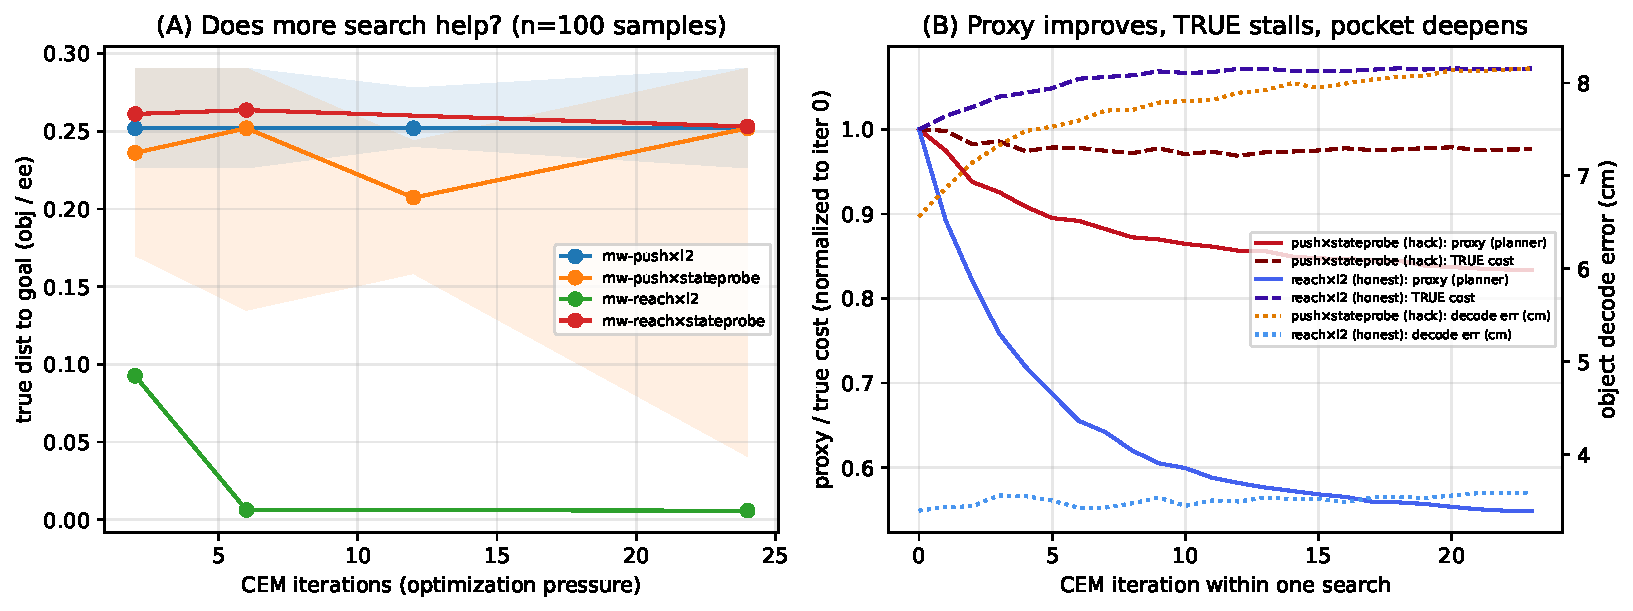
\includegraphics[width=\linewidth]{figures/figure_overopt.pdf}
\caption{\textbf{Cost overoptimization in latent planning.}
\emph{(A)}~True distance to goal vs.\ CEM iterations. reach$\times L_2$ (honest
cost) converts more search into success ($2/8\to8/8$); push$\times$probe-cost
(exploitable) and push$\times L_2$ (no-signal) do not improve with budget.
\emph{(B)}~Within one search at the largest budget, normalized to the first CEM
iteration: for push$\times$probe-cost the proxy the planner minimizes falls
($-17\%$) while the true state cost stalls ($-2\%$) and the object-decode error
on the committed elites \emph{grows} ($6.6\to8.2$\,cm, $+24\%$) --- the planner
digs into deeper readout-error pockets. The honest cost (reach$\times L_2$)
shows no such decode growth.}
\label{fig:overopt}
\end{figure}

The three predictions all hold (Fig.~\ref{fig:overopt}). \textbf{Exploitable
cost} (push, probe-based state cost): within a single search at budget $24$, the
believed-best candidate's proxy falls monotonically ($0.166\to0.138$, $-17\%$)
while its true object$\to$goal distance is flat ($0.279\to0.273$, $-2\%$) and the
probe's decode error on the elite population grows monotonically
($6.6\to8.2$\,cm, $+24\%$): more optimization, deeper pockets. Across budgets the
true object distance does not improve with search ($\mathrm{med}\approx0.25$\,m
at all of $\{2,6,12,24\}$ iterations; episode success stays within the frozen
band with CIs overlapping $0$). \textbf{Honest cost} (reach, $L_2$): the
essential positive control --- here more search \emph{does} convert to success
($2/8\to8/8\to8/8$ at $2/6/24$ iterations), confirming the sweep detects
``search helps'' when the cost is aligned. \textbf{No-signal cost} (push, $L_2$):
the proxy falls ($-32\%$) but the true object distance is \emph{exactly} flat
($0.252$\,m at every budget) --- $L_2$-in-latent has no minimum at task success,
so optimizing it is inert; this distinguishes an \emph{exploitable} cost (signal
present, worst-case reachable) from a merely \emph{uninformative} one. A second
pressure axis --- CEM population $\in\{50,100,300\}$ at fixed $12$ iterations ---
corroborates: enlarging the candidate pool does not improve the true push outcome
either (probe-cost median $0.233/0.207/0.252$\,m; $L_2$ flat).

\subsection{Mitigations from the playbook all fail}\label{sec:mitigations}
If the diagnosis is right, repairs that improve the cost's \emph{average}
quality without removing its \emph{worst-case} pockets should not cross the
wall --- the optimizer finds whatever pockets remain. We ran the standard
playbook, each arm under the latent oracle (perfect dynamics), push held-out,
strict success:

\begin{table}[h]
\centering\small
\caption{Mitigation ladder (latent oracle, push; 16 episodes per arm except the
learned-metric arm at 8). Every intervention that operates on or above a
frozen-base representation stays inside the frozen baseline's $0$--$2/16$ band
--- including those that push readout accuracy to near-ceiling. The true-state
cost row shows the same planner and budget solve the task when the cost has no
pockets.}
\label{tab:mitigations}
\begin{tabular}{llcc}
\toprule
intervention & grounding-level metric & push \\
\midrule
latent $L_2$ (frozen null) & --- & 0/16 \\
probe-based state cost & static decode 92\% $<$5\,cm & 2/16 \\
off-policy-hardened probes & off-policy 91.5\% $<$5\,cm & 1/16 \\
learned latent metric $d_\theta$ & --- & 0/8 \\
relearned repr.\ adapter $\varphi$ (v2) & held-out decode med.\ 6.9\,cm & 1/16 \\
encoder-LoRA + $\varphi$ (5 seeds) & decode 94--100\% $<$5\,cm & \{5,0,2,1,1\}/16; mean 1.8, CI $[0,3.7]$ \\
\;\;+ ensemble disagreement, $\lambda{\in}\{0,\tfrac12,1,2\}$ & --- & \{2,2,2,1\}/16 \\
\midrule
true-state cost (no pockets) & --- & \textbf{16/16} \\
\bottomrule
\end{tabular}
\end{table}

Three of these deserve comment. \textbf{Encoder fine-tuning} (LoRA on the
DINOv2 trunk, action-conditioned grounding objective, 5 seeds): grounding
reaches $94$--$100\%$, the five-seed planning mean is $1.8/16$ with CI
$[0,3.7]$ --- statistically inside the frozen band; the single $5/16$ seed is
high-variance noise, not a crossing. This is the strongest form of the paper's
recurring lesson: \emph{grounding does not buy planning}, now proven at the
encoder level, not just the readout level. \textbf{Ensemble disagreement}
(cost $= \mathrm{mean}_k d_k^2 + \lambda\,\mathrm{Var}_k[d_k]$ over 5
independently fine-tuned seeds) is the standard pessimism remedy for model
exploitation~\citep{janner2019trust}; it fails here ($\{2,2,2,1\}/16$ across
$\lambda$) for an instructive reason: the seeds share the frozen pre-trained
base, so they share the blind spot, and disagreement stays flat exactly on the
exploited pockets --- the same failure mode reported for reward-model ensembles
sharing a pre-trained trunk. \textbf{The state-oracle row} pins the counterfactual:
nothing about the task, budget, or planner prevents success; only the pockets do.

\paragraph{Summary of the mechanism section.}
A frozen-base learned cost, under test-time optimization pressure at
$100\times6$ candidates per replan, behaves like a reward model under
over-optimization: its average-case accuracy is irrelevant because the
optimizer samples from its worst case. Every repair that improves average-case
metrics --- readout precision, grounding, disagreement --- leaves the worst
case reachable. We were unable to produce a plannable post-hoc cost on a
frozen action-conditioned JEPA encoder for contact manipulation, across every
lever available to us; we conjecture, and our evidence supports, that
\textbf{any post-hoc cost on such an encoder is planner-exploitable at contact}.

% ======================================================================
\section{The axis that moves: counterfactual training of the predictor}
\label{sec:cf}

The ladder bypassed the predictor (perfect dynamics); the deployed stack still
uses one. Independently of the cost-side wall, the diagnostic of
Sec.~\ref{sec:diagnostic} identifies a training-target defect in the predictor:
under a teacher-forced objective, the target latent already contains the
action's effect, so the objective admits solutions in which the predictor
matches targets without using the action channel --- a mechanism independently
confirmed in a toy setting by~\citet{uwmjepa2026}. The corrective is to make
the objective \emph{counterfactual over actions}: the prediction under the
factual action must beat predictions under distractor actions, not just match
its target.

We instantiate this as an InfoNCE-over-actions objective on the frozen DROID
world model (\texttt{dino\_wm\_droid}): a predictor-LoRA of $0.469$M parameters
(encoder untouched, no object ground truth), trained so that
$F(z_t,a_t)$ scores higher against $z_{t+1}$ than $F(z_t,a^-_k)$ for
executed-action distractors $a^-_k$, with a stop-gradient on the target.
Counterfactual ranking accuracy rises $0.195\!\to\!0.736$ while reconstruction
\emph{improves} ($0.695\times$ baseline error) --- the objective is not trading
prediction quality for action sensitivity; it is removing a shortcut.

\begin{table}[h]
\centering\small
\caption{DROID planning probe, frozen vs.\ counterfactually-trained predictor
(A/B, same protocol, $n{=}157$ planned transitions; CEM $64\times15$). Action
Error = distance between the planned and the robot's executed action, in
normalized action units (lower is better); Action Score is the upstream
aggregate (higher is better); effect-CRA as in Sec.~\ref{sec:metrics} (chance
$\approx 0.059$). Action Error improves in all six regime$\times$horizon cells
(Action Score in 5/6); effect-CRA leaves the chance floor for the first time in
this paper.}
\label{tab:cf}
\begin{tabular}{llcccccc}
\toprule
 & & \multicolumn{2}{c}{Action Error $\downarrow$} & \multicolumn{2}{c}{Action Score $\uparrow$} & \multicolumn{2}{c}{effect-CRA $\uparrow$} \\
regime & $H$ & frozen & CF & frozen & CF & frozen & CF \\
\midrule
pre-grasp & 1 & 1.044 & \textbf{0.792} & 0.621 & \textbf{0.653} & 0.050 & \textbf{0.538} \\
gripper   & 1 & 1.080 & \textbf{0.577} & 0.607 & \textbf{0.748} & 0.000 & \textbf{0.583} \\
contact   & 1 & 1.267 & \textbf{0.950} & 0.539 & \textbf{0.584} & 0.125 & \textbf{0.575} \\
pre-grasp & 3 & 1.573 & \textbf{1.166} & 0.428 & \textbf{0.490} & 0.050 & \textbf{0.662} \\
gripper   & 3 & 2.208 & \textbf{1.571} & 0.197 & \textbf{0.313} & 0.045 & \textbf{0.727} \\
contact   & 3 & 1.907 & \textbf{1.661} & 0.307 & 0.273 & 0.118 & \textbf{0.529} \\
\midrule
pooled    &   & 1.468 & \textbf{1.086} & 0.466 & \textbf{0.525} & 0.061 & \textbf{0.605} \\
\bottomrule
\end{tabular}
\end{table}

\paragraph{The effect is robust to training seed, and transfers to a second
model.} Across four CF training seeds, the pooled improvement is tight and every
seed beats the frozen baseline on every metric: Action Error
$1.468\to1.076\pm0.012$, Action Score $0.466\to0.544\pm0.019$, effect-CRA
$0.061\to0.610\pm0.034$ (mean\,$\pm$\,sd over seeds; the single-seed column above
sits at the seed mean). On a second predictor family (\texttt{jepa\_wm\_droid}),
the objective lifts effect-CRA $0.076\to0.32$ and Action Score $0.476\to0.51$;
Action Error also improves ($1.386\to1.27$) once the LoRA rank is raised to $16$,
confirming the mechanism is not specific to one checkpoint.

Two readings, stated carefully. Positively: this is the predictor-axis repair
done at the correct level --- the training objective, not a post-hoc patch ---
and it produces the only across-the-board improvement of any intervention in
this paper, on real-robot data, without labels. Negatively: given
Sec.~\ref{sec:adversary}, we do \emph{not} claim this alone crosses the contact
wall in closed-loop planning --- the cost-side exploitation is untouched by a
better predictor (the ladder proved planning fails identically under
\emph{perfect} prediction). The two axes are complementary and both necessary;
conflating them is precisely the error the oracle ladder is designed to
prevent.

% ======================================================================
\section{Discussion, scope, and limitations}\label{sec:discussion}

\paragraph{What follows for evaluation.}
Every quantity the field currently reports was satisfied at some rung of this
paper while planning failed: held-out prediction error (Sec.~\ref{sec:planning}
harness on-manifold), action grounding ($94$--$100\%$ in
Table~\ref{tab:mitigations}), readout precision ($91.5\%$ within $5$\,cm on the
planner's own query distribution). The quantity that tracked the failure
throughout is the \emph{exploitation gap}: the discrepancy between the cost's
claim and the world's truth \emph{on the states the optimizer converges to}
(Table~\ref{tab:exploit}, and the overoptimization curves of
Fig.~\ref{fig:overopt}). We propose reporting it
directly: mine the planner's elite population and decode it against ground
truth (in sim), or against a held-out verifier (on real data). It is cheap ---
one extra decode pass over frames the planner already produced.

\paragraph{What follows for method design.}
The results sort the design space into three responses. (i)~\emph{Harden the
cost}: our evidence says this loses on frozen-base representations --- average
metrics improve, worst-case pockets remain, the optimizer finds them
(Table~\ref{tab:mitigations}). (ii)~\emph{Fix the training objective}: the
counterfactual objective (Sec.~\ref{sec:cf}) is the right lever for the
predictor axis, and encoder-level analogues remain open --- but grounding alone
demonstrably does not buy planning. (iii)~\emph{Remove the adversary}: if
test-time search is what weaponizes cost error, amortizing planning into a
policy or inverse-dynamics controller~\citep{latentgeom2026}, or anchoring the
search to demonstration priors~\citep{imwm2026}, removes the optimization
pressure rather than the pockets. We tested this directly (Sec.~\ref{sec:e1}):
a goal-conditioned inverse-dynamics controller built from the same frozen
representation and readout, run with \emph{no} search, and the same controller
with search re-added in increasing doses. The result is a null and it sharpens
the paper's claim rather than softening it --- see below.

\paragraph{Removing the adversary is necessary, not sufficient.}\label{sec:e1}
Under the latent oracle on push, the search-free amortized controller solves
$0/8$, and every re-added search dose (CEM iterations $\{0,2,6,12,24\}$ seeded
from the controller) also solves $0/8$; in all arms the object never leaves its
start ($\mathrm{med}\ \|obj-goal\|\approx0.25$\,m, Fig.~\ref{fig:e1}A). Removing
the optimizer does not cross the wall. Two things are nonetheless confirmed. On
the mechanism side, the per-replan seed-vs-chosen comparison shows search
``improves'' the proxy over the seed on $98$--$100\%$ of replans while
\emph{corrupting} the true state (proxy down, truth up) on a fraction that rises
monotonically with dose ($0\to7\%$, Fig.~\ref{fig:e1}B) --- the adversary is real
and dose-dependent even here. But it is not the \emph{only} wall: a controller
with no optimizer to exploit it still fails, because the frozen representation
and its object readout do not carry a plan that moves the object. The honest
synthesis across the oracle ladder, the mitigation table, and this experiment is
that contact planning faces \emph{two} walls --- an exploitable cost/optimizer
interface (E0, Secs.~\ref{sec:ladder}--\ref{sec:overopt}) and an insufficient
frozen representation (E1) --- and that \emph{grounding is necessary but not
sufficient}: neither hardening the cost, nor fine-tuning the encoder for
grounding, nor removing the search adversary, crosses it alone.

\begin{figure}[t]
\centering
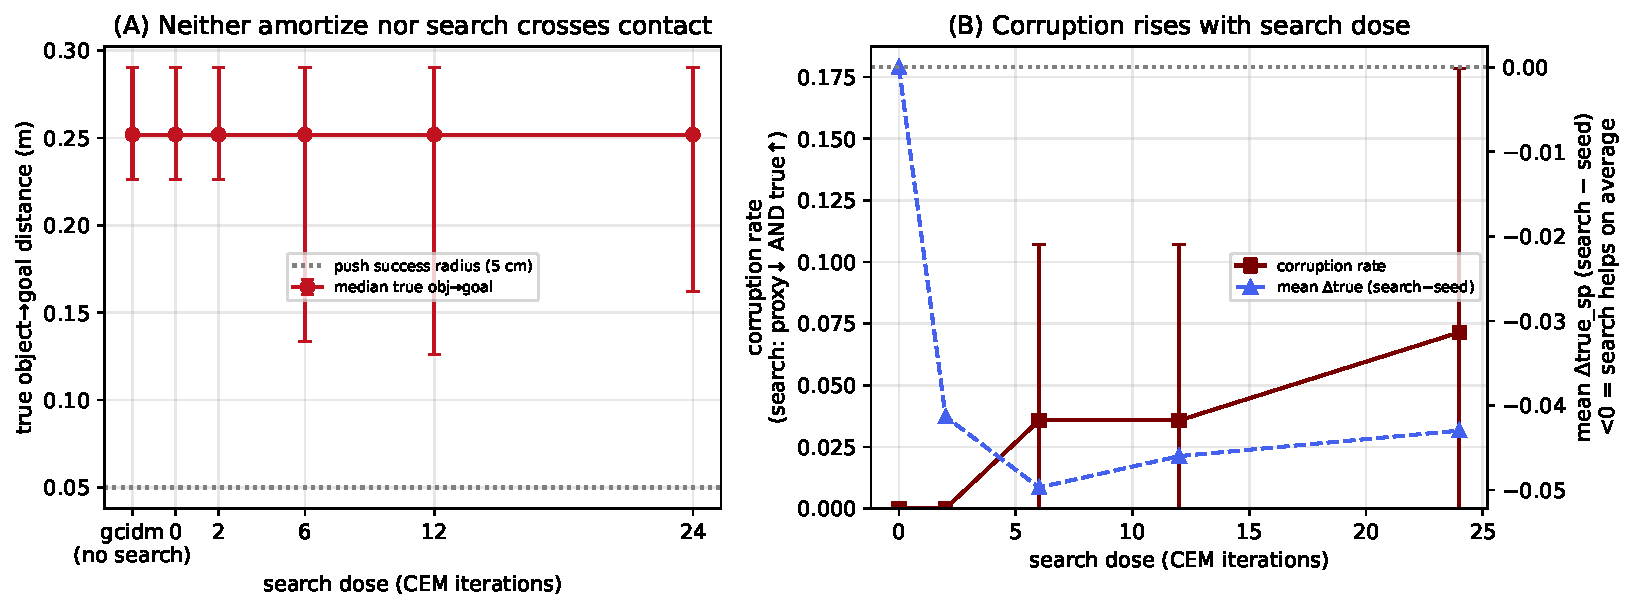
\includegraphics[width=\linewidth]{figures/figure_e1.pdf}
\caption{\textbf{Removing the search adversary does not cross contact (E1).}
\emph{(A)}~True object$\to$goal distance for the pure amortized controller
(``gcidm'', no search) and for search re-added in doses; all sit at
$\approx0.25$\,m, far above the $5$\,cm success radius. \emph{(B)}~Per-replan
corruption rate (search lowers the proxy \emph{and} raises the true cost) rises
with search dose ($0\to7\%$), while the mean true-cost change from search stays
negative (on average search still helps the \emph{hand}) --- the adversary is
real but small, and the object never moves regardless.}
\label{fig:e1}
\end{figure}

\paragraph{Scope and honest limits.}
The exploitation mechanism is established on Metaworld, where simulator state
lets us verify every claim against ground truth; on DROID we establish the
diagnostic (scale-flat chance-floor grounding) and the predictor-axis repair,
but closed-loop exploitation curves on real robots remain future work. The
mitigation table covers the levers available on frozen pretrained checkpoints
(readouts, metrics, adapters, LoRA fine-tuning, ensembles); full encoder
retraining with planner-aware objectives is beyond our compute and remains
open --- our claim is about the \emph{post-hoc} regime. The boundary-regime
labels use an object-displacement proxy (no MuJoCo contact ground truth in the
released data); mw-door-close is excluded as a proxy anomaly. The Reach parity
check compares one released checkpoint over 16 episodes against a published
3-seed$\times$96-episode number --- we read it as ``reproduces, inside the CI'',
not a seed-matched replication. Finally, an information-sufficiency question
remains open beneath everything: vision-only latents may lack contact state
outright~\citep{contactworld2026}; our state-oracle row shows the \emph{task}
is solvable from privileged state, but whether any vision-only cost can be made
pocket-free is not settled by this paper.

\section{Conclusion}
Contact-rich planning with JEPA world models does not fail for want of encoder
scale, prediction accuracy, grounding, or readout precision --- all were
satisfied, measured, at some rung of our ladder while push stayed at $0$--$2/16$.
It fails because a test-time optimizer is pitted, hundreds of candidates per
control step, against a learned cost whose residual-error pockets it is
structurally guaranteed to find --- and the same planner solves the same task
$16/16$ the moment the cost has no pockets. Repairs aimed at the average case
(hardened readouts, fine-tuned encoders, ensembles) leave the worst case
reachable; the training-side objective that repairs the predictor's action
channel is real and label-free but orthogonal to the cost-side wall. World
models intended for planning should be evaluated the way their planners attack
them: not by how well they predict, but by how little they can be exploited.

\bibliographystyle{plainnat}
\bibliography{refs}

\appendix
\section{Boundary Blindness: definition}\label{app:bb}
The instrument compares, on a neighbourhood of similar states, how much the
\emph{world's} outcome fans out under nearby actions against how much the
\emph{model's} prediction fans out under the same actions.

\paragraph{Neighbourhood.} For each anchor transition $i$ with latent $z_i$ and
action $a_i$, $\mathcal{N}(i)$ is its $M{=}16$ nearest cached transitions in
latent distance, radius-limited with relaxation (the same neighbourhood the
hard-negative CRA sampler uses). $o_j$ is the true scalar outcome of neighbour
$j$: object displacement $\|\Delta\mathrm{obj}_j\|$ on Metaworld, the
$\|\Delta z_j\|$ proxy on DROID.

\paragraph{Boundary regime.} A transition is \emph{boundary} when small action
changes produce large true-outcome changes across its neighbourhood:
\begin{equation}
  \mathrm{boundary\_score}_i =
  \frac{\operatorname{std}_{j}\, o_j}
       {\operatorname{mean}_{j} \|a_j - a_i\| + \varepsilon},
\end{equation}
thresholded at a population percentile. Free-space drift has large $\|\Delta z\|$
but smooth neighbourhoods and scores low.

\paragraph{The two sensitivities and BB.} The world's local action-sensitivity
$S^{\mathrm{true}}_i$ is the dispersion of true outcomes across the
neighbourhood; the model's, $S^{\mathrm{model}}_i$, applies each neighbour's
action to the \emph{single} anchor state and measures the RMS spread of
$F(z_i, a_j)$ around its centroid. Each is z-scored over the population and
\begin{equation}
  \bb_i = \operatorname{relu}\big(\tilde S^{\mathrm{true}}_i
                                 - \tilde S^{\mathrm{model}}_i\big),
\end{equation}
pooled ($n_b$-weighted) over the boundary mask with trajectory-clustered
bootstrap CIs. Because BB references the world, a high value cannot be an
artefact of small one-step latent deltas.

\section{The grounded-channel fix ladder (metric-level repair)}
\label{app:fixladder}
Deferred from Sec.~\ref{sec:planning}: the model-side repair ladder that
motivated the oracle ladder. \textbf{Nulls:} mixture-density predictor heads
(soft-NLL/WTA/hard-EM/supervised, $K{\in}\{2,3\}$) beat their $K{=}1$ NLL
controls but do not move $\bb_{\mathrm{boundary}}$ --- the bifurcation spans
$9.9$ $L_2$ units against a $106$ median residual (the geometry under-weights
the boundary subspace $10\times$), and the boundary's action-dependence is
unlearnable from expert-only data at the head level. Probe-subspace metric
re-weighting redistributes BB without reducing it. \textbf{The probe chain:}
object state is decodable from the frozen latent (V1 err $0.064$ vs.\ sd
$0.094$), propagates through the predictor for \emph{factual} actions (V2
$0.059$), but the \emph{counterfactual} action$\to$object response is noise (V3
spread-corr $+0.035$). \textbf{The repair:} a $0.5$M grounded dynamics channel
$h(z_t,a)\!\to\!\widehat{\Delta\mathrm{obj}}$ (mean/max-pooled tokens + action
MLP), trained on cached latents with everything frozen, restores counterfactual
tracking ($0.035\!\to\!0.682$ DINO-WM; $0.702$ JEPA-WM), halves boundary BB on
both families ($1.323\!\to\!0.660$; $1.280\!\to\!0.620$), and improves the
closed-loop cost surface (Table~\ref{tab:closedloop}) --- while flipping zero
successes, the observation Sec.~\ref{sec:ladder} explains. Honest negative: the
recipe does not transfer to DROID's noisy whole-state proxy label at $2.1$k
transitions (rank-corr $+0.708$ but spread magnitude collapsed; BB unchanged) —
the principle needs a learnable grounding label.

\section{Reproduction integrity}\label{app:repro}
Closed-loop sim evaluation is fragile, and getting the baseline wrong would
invalidate the parity argument. Three environment-side bugs, found and fixed,
all model-agnostic: \textbf{(1)}~Metaworld's offscreen renderer is constructed
in the env constructor, so camera/size assignments afterwards were silently
ignored (default camera at $480$\,px vs.\ the trained \texttt{corner2} at
$224$\,px; symptom: one-step prediction error $8.5\times$ dataset level). We
re-create the renderer explicitly, mirroring the upstream wrapper.
\textbf{(2)}~The released training frames are vertically flipped relative to
today's \texttt{corner2} render; pixel-calibration against dataset initial
frames scores the flipped wrapper-camera render at MSE $71.6$ vs.\ $\geq 3000$
for every unflipped candidate. \textbf{(3)}~The success flag fires at a
$5$\,cm radius but the scripted expert refines to $\sim$1\,cm; taking the goal
frame at first-success rather than the expert's final frame parked the planner
just outside the radius. \textbf{Verification:} after the fixes, one-step
prediction error is $1.4\times$ dataset level, latent NN ratio $0.97$, and
replaying dataset actions reproduces the proprioceptive trajectory to
$1.5$\,mm median end-effector error --- only the visuals had drifted, never the
physics. The reach baseline then recovers from near-zero to $37.5\%$
(Table~\ref{tab:closedloop}), inside the published CI.

\section{AUG and ECS: the raw-gap corroboration}\label{app:augecs}
CRA leads the main text because, as a ranking, it is cross-model comparable.
The two raw-gap metrics corroborate it: AUG (prediction-error gap between
permuted and factual actions; $\approx 0$ iff actions ignored) and ECS (AUG on
effect-bearing transitions), both on the hard nearest-neighbour family.

\begin{table}[h]
\centering\small
\caption{AUG\,/\,ECS, hard nearest-neighbour family, per regime
($n_{\mathrm{eff}}$-weighted pools; dash = no effect-bearing transitions). Raw
latent gaps are \emph{not} comparable across models (latent scales differ); the
cross-model statement lives in CRA (Tables~\ref{tab:cra},~\ref{tab:scaling}).}
\label{tab:augecs}
\begin{tabular}{lcccc}
\toprule
model & free space & pre-grasp & gripper & contact \\
\midrule
\multicolumn{5}{l}{\emph{DROID} (real robot; AUG\,/\,ECS)}\\
DINO-WM (22M)        & 0.038/-- & 0.011/0.0105 & 0.038/0.0645 & 0.070/0.0094 \\
JEPA-WM (300M)       & 0.000/-- & 0.000/0.0002 & 0.001/0.0004 & 0.001/$-$0.0011 \\
V-JEPA-2-AC (1B)     & 0.006/-- & 0.002/0.0016 & 0.003/0.0026 & 0.003/$-$0.0059 \\
V-JEPA-2-AC-OSS (1B) & 0.004/-- & 0.001/0.0010 & 0.001/0.0005 & 0.003/$-$0.0030 \\
\midrule
\multicolumn{5}{l}{\emph{Metaworld} (sim; AUG\,/\,ECS; pooled over 12 tasks)}\\
DINO-WM (22M)        & 0.088/0.1007 & 0.051/0.0997 & --/-- & 0.081/0.0893 \\
JEPA-WM (300M)       & 0.089/0.1020 & 0.058/0.1114 & --/-- & 0.095/0.1052 \\
\bottomrule
\end{tabular}
\end{table}

\noindent The effect-conditioned action gap is statistically indistinguishable
from zero on the real-robot data across the full $45\times$ scale range ---
the chance-level CRA reflects genuine action-ignoring, not a ranking quirk.
Source: \texttt{results/\{droid,metaworld\}\_diagnostic.csv}, \texttt{hard\_nn}
rows.

\section{Full per-task tables}
\todo{per-task BB CSV dumps; mitigation-arm episode tables (phaseC/D/F/G logs);
E0 curve tables when jobs 24740/24741 land; Phase-H seed-sweep CIs.}

\end{document}
